\documentclass[twocolumn, 11pt]{article}
\usepackage{amsmath, graphicx, xcolor, fancyhdr, tocloft, soul}
\usepackage[colorlinks=true, linkcolor=black, urlcolor=blue, citecolor=black]{hyperref}
\usepackage{tikz}
\usetikzlibrary{shapes.geometric, arrows.meta, positioning}


% Color for titles
\definecolor{darkpurple}{RGB}{102, 0, 153}

% Fancy header and footer
\pagestyle{fancy}
\fancyhf{}
\lfoot{\textit{Project 2 Report}}
\cfoot{\thepage}

\renewcommand{\headrulewidth}{0pt}
\renewcommand{\footrulewidth}{0.4pt}

% Modify title format to use dark purple
\makeatletter
\renewcommand{\maketitle}{\bgroup
  \centering
  {\LARGE \bfseries \color{darkpurple} \@title \par}
  \vskip 1em
  {\large \color{darkpurple} \@author \par}
  \vskip 1em
  {\footnotesize \@date \color{darkpurple}\par}
  \egroup
}
\makeatother

% Color for section titles and uniform size for section and subsection
\usepackage{titlesec}
\titleformat{\section}
  {\normalfont\large\bfseries\color{darkpurple}}
  {\thesection}{1em}{}

\titleformat{\subsection}
  {\normalfont\large\bfseries\color{darkpurple}}
  {\thesubsection}{1em}{}

% Document title (Single-column)
\title{Simulation of Uranium-235 Fission in a Sealed Water Tank}
\small\author{\small Kevin Mesta, Sara Talebi \\ \small Department of Chemistry, Syracuse University, Syracuse, New York 13244 USA}
\date{October 2024}

\begin{document}

% Switch to a single column for title, author, and date
\twocolumn[
\begin{@twocolumnfalse}
    \maketitle
    \vspace{10pt}
\end{@twocolumnfalse}
]

% Now we switch back to two-column for the rest of the document
\section*{Introduction}
This project involves simulating the behavior of uranium-235 (U-235) particles in a sealed water tank, focusing on neutron-induced fission reactions and the subsequent energy transfer to the surrounding water. The simulation includes the following key elements:
\begin{itemize}
    \item Neutron-induced fission of U-235.
    \item Movement and heat transfer of particles in water.
    \item Tracking temperature changes in the water due to energy released from fission reactions and drag .
    \item Tracking individual neutrons and their interactions with U-235.
    \item Monitoring the total mass and particle counts resulting from fission reactions.
\end{itemize}

\section*{Boundary Conditions}
The simulation incorporates the following boundary conditions:
\begin{itemize}
    \item \textbf{No heat loss by the tank}: The tank is perfectly insulated, so all energy released by fission reactions is transferred to the water, raising its temperature.
    \item \textbf{Particle-wall interactions}: When particles collide with the tank walls, they lose no energy but change their direction of motion.
    \item \textbf{Neutron-wall interactions}: Neutrons scatter off the walls elastically, with no energy loss, and change their direction of motion.
    \item \textbf{Particle-particle interactions}: Particles collide elastically, conserving momentum and scattering in random directions.
\end{itemize}

\section*{Simulation Methodology}
The simulation follows these key steps:

\begin{itemize}
    \item \textbf{Particle Initialization:} The simulation begins with a set number of neutrons and uranium particles randomly placed inside a well-defined cubed water tank according to an exponential distribution. Each particle is assigned an initial velocity depending on its type (e.g., neutrons have higher velocities than uranium).
    
    \item \textbf{Particle Movement:} Particles move at each time step symplectically according to their velocity at the next time step and are affected by drag forces due to water. The drag force is a resistive force, reducing the velocity over time according the following second order ODE:
        \[
        0 = m\frac{d^{2}x}{dt^{2}} - \frac{1}{2}C_{d}\rho A (\frac{dx}{dt})^2
        \]
    where m represents the mass of the particle traveling through water, \mathrm$C_{d}$ is the drag coefficient, rho is the density of water and A is the cross sectional area of the spherical particles in this case.
    
    \item \textbf{Collisions:} The simulation checks for particle-wall and particle-particle collisions at each time step. Particles scatter elastically off the tank walls, while particle-particle interactions can result in elastic collisions or fission reactions, depending on the particle types involved. Particles are said to be in a collision if they are within a certain distance from one another proportional to the sum of both particle's radii. 
    
    \item \textbf{Fission Reactions:} When a neutron collides with a uranium particle, a fission event occurs, destroying the uranium atom and neutron particle associated with the fission event and producing one krypton atom, one barium atom, and three new neutrons. The energy released in the fission event set is tracked and used to calculate the temperature change in the water.
    
    \item \textbf{Energy and Heat Transfer:} Energy from fission reactions and drag forces is accumulated and used to compute the temperature increase in the water, assuming no heat loss to the environment(outside the tank).
\end{itemize}

% First Flowchart: General Simulation Flow
\begin{figure}[h!]
\centering
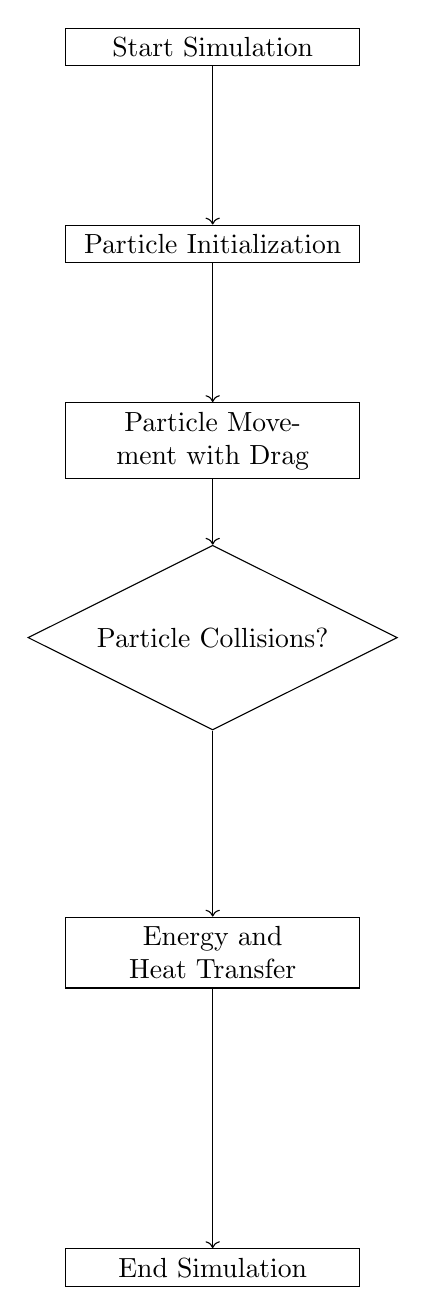
\begin{tikzpicture}[node distance=2.5cm, auto]

% Nodes
\node (start) [rectangle, draw, text width=3.5cm, align=center] {Start Simulation};
\node (init) [rectangle, below of=start, draw, text width=3.5cm, align=center] {Particle Initialization};
\node (move) [rectangle, below of=init, draw, text width=3.5cm, align=center] {Particle Movement with Drag};
\node (collision) [diamond, below of=move, draw, aspect=2, text width=3.5cm, align=center] {Particle Collisions?};
\node (energy) [rectangle, below of=collision, yshift=-1.5cm, draw, text width=3.5cm, align=center] {Energy and Heat Transfer};
\node (stop) [rectangle, below of=energy, yshift=-1.5cm, draw, text width=3.5cm, align=center] {End Simulation};

% Arrows
\draw[->] (start) -- (init);
\draw[->] (init) -- (move);
\draw[->] (move) -- (collision);
\draw[->] (collision) -- (energy);
\draw[->] (energy) -- (stop);

\end{tikzpicture}
\caption{Flowchart of General Simulation Flow: Particle Movement, Collision, Energy Transfer, and End}
\end{figure}

\section*{Sampling Using the Inverse CDF Method}

In our simulation, we utilized the \textit{Inverse Cumulative Distribution Function (CDF)} method for random sampling to generate initial particle velocities and positions. This approach allows us to sample from a desired probability distribution by transforming uniform random variables into variables that follow the distribution of interest.

The \textbf{probability density function (PDF)} of the exponential distribution is given by:

\[
f(x; \lambda) = \lambda e^{-\lambda x} \quad \text{for} \quad x \geq 0
\]

where \( \lambda \) is the rate parameter.

The \textbf{cumulative distribution function (CDF)} of the exponential distribution is:

\[
F(x) = 1 - e^{-\lambda x} \quad \text{for} \quad x \geq 0
\]

The CDF represents the probability that a random variable \(X\) takes a value less than or equal to \(x\), i.e., \( P(X \leq x) = F(x) \).

The inverse CDF method allows us to generate random samples from the exponential distribution. Here’s how it works:
\begin{enumerate}
    \item Generate a random uniform value \( U \) from the interval \( [0, 1] \).
    \item Set \( x = F^{-1}(U) \), where \( F^{-1} \) is the inverse of the CDF. For the exponential distribution, the inverse CDF is:
\end{enumerate}

\[
x = -\frac{1}{\lambda} \ln(1 - U)
\]

Since \( U \) is a uniform random number, this equation transforms it into a random variable \( x \) that follows the exponential distribution.

In our simulation, we applied the inverse CDF method to sample initial velocities for the neutrons and uranium particles. Using the inverse CDF method provides an efficient and straightforward way to sample from non-uniform distributions, enabling us to model particle behavior more realistically in our fission simulation.

\section*{Physical Background}
The simulation models neutron-induced fission in uranium-235 (\(^{235}\text{U}\)), a common reaction in nuclear reactors. When a neutron (\(n\)) collides with a \(^{235}\text{U}\) nucleus, it splits into two smaller nuclei (typically barium and krypton), releases a large amount of energy, and emits additional neutrons that can propagate further fission reactions, initiating a chain reaction.

The simplified chemical equation for this fission process is:

\[
^{235}\text{U} + n \rightarrow ^{141}\text{Ba} + ^{92}\text{Kr} + 3n + \text{Energy}
\]

Energy refers to the energy released in the form of the kinetic energy of the fission products, typically around \(200 \, \text{MeV}\) per fission event.

Each fission reaction releases approximately \(2.97 \times 10^{-11}\) joules of energy, which is transferred to the surrounding water. This energy heats the water and can be used to simulate temperature changes over time, as we have done in this project.

\section*{Results}
The simulation was run with four neutrons and two uranium-235 particles inside a 1-meter cubed water tank, with the initial water temperature set to 25°C.

\textbf{Initial particle counts:}
\begin{itemize}
    \item Neutrons: 4
    \item Uranium: 2
    \item Barium: 0
    \item Krypton: 0
\end{itemize}

During the simulation, two fission reactions occurred:
\begin{itemize}
    \item Each reaction created one barium, one krypton atom, and three neutrons.
    \item A total of 2 uranium atoms and 2 neutron particles were consumed.
    \item The particle count at the end of the simulation was:
        \begin{itemize}
            \item Neutrons: 8
            \item Uranium: 0
            \item Barium: 2
            \item Krypton: 2
        \end{itemize}
\end{itemize}

\textbf{Note:} We observed that the initial probability of particle collisions was very low due to the small size of the particles relative to the simulation space. To account for this, we introduced a threshold for the minimum distance between two particles (\(1 \times 10^{-9}\) meters) to increase the likelihood of collisions. This artificial threshold is justified by the need to ensure meaningful interactions within the limited number of particles in the simulation. While this approach increases the collision chances, it also slightly affects the physical accuracy of the simulation, as it allows particles to interact at a distance where they might not collide in reality.

\subsection*{Heat Release and Temperature Change Analysis}
To further investigate how the number of uranium-235 atoms affects the temperature of the surrounding water, we conducted simulations with different quantities of uranium atoms, ranging from 1 to 1000. The simulation used a consistent number of neutrons (4), a cubic water tank length of 1 meter and assumed that the initial temperature of the water was 25°C. 

For each simulation, we tracked the temperature change in the water due to the energy released from fission reactions and drag forces. The resulting temperature changes were plotted as a function of the number of uranium atoms, as shown in Figure \ref{fig:heat_release}.

\begin{figure}[h]
    \centering
    \includegraphics[width=\linewidth]{temp_change_vs_uranium.png}
    \caption{Temperature Change as a function of the Number of Uranium Atoms in the simulation.}
    \label{fig:heat_release}
\end{figure}

As can be seen from the graph, there is a clear positive relationship between the number of uranium atoms and the temperature change in the water. Initially, the temperature change is relatively small with small numbers of uranium atoms. However, as the number of uranium atoms increases, we observe a more significant temperature rise, with the most considerable jump occurring between 700 and 1000 uranium atoms.

This behavior aligns with expectations, as more fission reactions lead to greater energy release, contributing to a higher water temperature. The temperature change, though small in magnitude due to the large volume of water and small number of uranium atoms in each simulation, directly correlates with the fission events.

In addition to varying the number of uranium atoms, we also explored the effect of the simulation's box size on the temperature change in the water. Specifically, we reduced the box size from \(1 \, \text{m}^3\) to \(1 \, \text{cm}^3\), keeping all other parameters constant (including the number of neutrons and uranium atoms). 

This significant reduction in volume increases the energy density, meaning that the same amount of energy is released into a much smaller space, leading to more pronounced temperature changes. Figure \ref{fig:small_box_heat_release} shows the temperature change as a function of the number of uranium atoms in this smaller box.

\begin{figure}[h]
    \centering
    \includegraphics[width=\linewidth]{temp_change_vs_uranium_1cm.png}
    \caption{Temperature Change as a function of the Number of Uranium Atoms in a \(1 \, \text{cm}^3\) simulation box.}
    \label{fig:small_box_heat_release}
\end{figure}

As expected, reducing the box size leads to a much greater temperature change for the same number of uranium atoms. For example, with 1000 uranium atoms, the temperature increases by a factor of a billion, compared to when the simulation was performed in a 1-meter cubed box. This is consistent with deceasing the volume by a factor of one billion the same amount of heat in the smaller box leads to a more pronounced temperature change.

This result illustrates the significant impact of spatial confinement on heat dissipation. In real-world applications, such as reactor design, spatial constraints are crucial in determining how energy is distributed and how quickly systems heat up. The larger temperature changes observed in this smaller box underscore the importance of system size when simulating or designing nuclear reactors and when considering safety mechanisms to manage heat.

To further explore the effect of box size on the temperature change, we reduced the box size to \(8 \, \mu\text{m}^3\) and simulated the temperature change for uranium atom counts ranging from 1 to 25. This configuration allowed us to investigate how extreme spatial confinement affects energy distribution and heat dissipation in the system.

The resulting heatmap (Figure \ref{fig:heatmap_analysis}) shows the temperature change in the water as a function of both the number of uranium atoms and the small box size. The heatmap reveals that as the number of uranium atoms increases, the temperature change becomes much more pronounced, rapidly reaching extreme levels due to the confined space.

\begin{figure}[h]
    \centering
    \includegraphics[width=\linewidth]{final_heatmap.png}
    \caption{Heatmap showing temperature change (°C) as a function of the number of uranium atoms and a box size of \(8 \, \mu\text{m}^3\).}
    \label{fig:heatmap_analysis}
\end{figure}

In this scenario, with as few as 20 uranium atoms, the temperature rises to over 200°C. This result highlights the extreme sensitivity of temperature to both particle count and volume reduction. The concentration of energy in such a small space leads to far more significant heating compared to the larger box sizes analyzed earlier.

This analysis demonstrates that when simulating fission reactions in very small volumes, the temperature rise can become extreme, even with relatively small numbers of uranium atoms. This result could have implications for high-density reactor designs or micro-reactor applications, where controlling heat dissipation becomes critically important. The rapid temperature rise observed in such small volumes also highlights the potential dangers of spatial confinement in nuclear reactions.


\section*{Performance and Bench-marking}
We conducted benchmarks to assess the performance of the simulation with varying numbers of particles and time steps. As expected, increasing the number of particles increased the computational load due to more particle-particle interactions, particularly for collision detection. The most significant computational cost is associated in the principal simulation command that loops through all particles in the simulation and for each particle it checks all other particles within the simulation. The overall big O notation is then O(\mathrm$n^2$) where n is the number of particles in the simulation. 

 This time complexity can be observed when running simulations for varying number of neutrons or uranium atoms as seen in the figures that follow. In Figure \ref{fig:neutron_time_analysis} the average simulation time for 5 simulations of a given neutron count is plotted against the neutron range. Visually inspecting the plot there is an exponential relationship between the number of neutrons and the simulation time. Specifically, when there are 500 neutrons the simulation time is approximately 0.25s and doubling the amount of neutrons to 1000 causes the simulation time to jump to approximately 1.0s. This can be seen when going from 200 to 400 neutrons as the time changes from 0.05s to 0.2s.           

\begin{figure}[h]
    \centering
    \includegraphics[width=\linewidth]{sim_time_vs_neurtrons.png}
    \caption{Graph of simulation time for varying number of neutrons in a box size of \(1 \,\text{m}^3\), 2 initial uranium atoms and a time step of 0.001 seconds}
    \label{fig:neutron_time_analysis}
\end{figure}

In Figure \ref{fig:uranium_time_analysis} the simulation time for varying numbers of uranium atoms is plotted with a similar shape to that in the previous figure. The average simulation time for 300 uranium atoms is approximately 10 seconds and when jumping to 600 uranium atoms average simulation time is approximately 40 seconds, exhibiting the expected relationship between computation time and the number of particles. The principal difference is that increasing the number of uranium atoms drastically increases the computation time for the simulation due to the nature of the model. For each uranium atom that is added, an additional 3 particles are added to the simulation when a fission event occurs. This causes the time complexity to remain O(\mathrm$n^2$) but with a larger constant. 

\begin{figure}[h]
    \centering
    \includegraphics[width=\linewidth]{sim_time_vs_uranium.png}
    \caption{Graph of simulation time for varying number of uranium atoms in a box size of \(1 \,\text{m}^3\), 4 initial neutron particles and a time step of 0.001 seconds}
    \label{fig:uranium_time_analysis}
\end{figure}

Additionally, the effect of the time step on the average temperature change and simulation time was investigated. The average temperature change with respect to time step did vary across different step sizes but was not drastically different. This can be seen in Figure \ref{fig:temp_dt_analysis} with the temperature change staying relatively consistent and the higher temperature at smaller time steps is most likely attributed to a better determination of energy transferred to surrounding water due to force of drag. 

\begin{figure}[h]
    \centering
    \includegraphics[width=\linewidth]{temp_change_vs_dt.png}
    \caption{Graph of average temperature change across 25 simulations for varying number of time steps in a box size of \(1 \,\text{m}^3\), 4 initial neutron particles and 2 uranium atoms}
    \label{fig:temp_dt_analysis}
\end{figure}

The effect that time step has on average simulation time can be determined intuitively but is further supported by Figure \ref{fig:time_dt_analysis}. At smaller time steps, the average simulation time is greater due to more computational time step determining where all particles are. This may also lead to the determination of more accurate collisions between particles but does create a greater time demand. 

\begin{figure}[h]
    \centering
    \includegraphics[width=\linewidth]{sim_time_vs_dt.png}
    \caption{Graph of average simulation time across 25 simulations for varying number of time steps in a box size of \(1 \,\text{m}^3\), 4 initial neutron particles and 2 uranium atoms}
    \label{fig:time_dt_analysis}
\end{figure}

\section*{Validation}
The fission reactions resulted in the expected particle transformations (production of krypton, barium, and neutrons). The particle interactions and elastic collisions followed momentum conservation, and no particles escaped the tank or lost energy during wall collisions, consistent with the boundary conditions.

We compared the energy before and after each particle collision to validate the simulation to ensure momentum and energy conservation. Additionally, we compared the fission yield (three neutrons per fission) with known values from the literature. The results showed good agreement, indicating that the physical behavior is correctly modeled.

\textbf{Energy Conservation:}

The principal form of energy conservation was in the elasticity of particle collisions involving non neutron-uranium pairs. In these cases the total momentum of two particles colliding in the the x, y, and z directions was optionally displayed in the elasticCollision method. These optional print statements prove that the total momentum before and after colliding was indeed conserved.

However, there is a case in which the velocity of a particle becomes increasingly small and so determining the new velocities to maintain the total momentum is no longer feasible. This is due to the finite precision of simulating particles and their velocities and this causes errors at extremely small value. In this instance, the velocities are swapped and then particles are scattered in a random direction in order to best maintain momentum.

\textbf{Mass Conservation:}
The conservation of mass is another aspect of validation within the simulation environment, ensuring that no methods produce an inaccurate amount of particles and is therefore as close to the expected behavior. This was done by determining the initial mass of the system when the particles are initially generated and then once the last uranium atom has reacted determining the final mass of the system. In all instances the mass initially and the final mass are both equal to one another ensuring that mass is conserved.

\section*{Error Analysis}
The simulation involves multiple sources of numerical error, including:
\begin{itemize}
    \item Discretization error in the time-step (\(\Delta t = 1 \text{ ms}\)).
    \item Rounding error in floating-point arithmetic, especially when dealing with small energy changes.
    \item Sampling error introduced by probabilistic interactions.
\end{itemize}



Using sufficiently small time steps kept in check finite precision and time-stepping errors, but more accurate bench-marking would be needed to quantify these effects in detail. The numerical error(floating point error) presented in multiple instances, from particle collisions and velocity updates, and was dealt with as described in relevant sections. However, this numerical error is not able to be mitigated fully and as such there is always an inherent numerical error present throughout the simulation. 

In order to verify the amount of 
\begin{figure}[h]
    \centering
    \includegraphics[width=\linewidth]{avg_avg_temp.png}
    \caption{Graph of the average of the average temperature change of a varying number of simulations repeated 100 times in a box size of \(1 \,\text{m}^3\), 4 initial neutron particles and 2 uranium atoms and time step of 0.001 seconds}
    \label{fig:avg_avg_analysis}
\end{figure}
sampling error found within the simulation the following procedure was followed. For a fixed set of initial conditions the simulation was repeated 10, 25, 50, 75, 100, 200, 300, 400, and 500 times and the average temperature change and corresponding standard deviation of temperature change was determined. This was then repeated 100 times for each simulation size resulting in an average of average temperature change and a standard deviation of average temperature change with the results shown in Figures \ref{fig:avg_avg_analysis} and \ref{fig:stdev_avg_analysis} below.
In Figure \ref{fig:avg_avg_analysis} the average of the average temperature change is plotted against the size of the simulation batch. From this graph we can see that average temperature change is approximately 1.50e-16 as most of the simulation batches hover around this value. What is of importance is that in Figure \ref{fig:stdev_avg_analysis} the standard deviation of the average temperature change decreases as the size of 
\begin{figure}[h]
    \centering
    \includegraphics[width=\linewidth]{stdev_avg_temp.png}
    \caption{Graph of the standard deviation of the average temperature change of a varying number of simulations repeated 100 times in a box size of \(1 \,\text{m}^3\), 4 initial neutron particles and 2 uranium atoms and time step of 0.001 seconds}
    \label{fig:stdev_avg_analysis}
\end{figure}
 the simulation batch increases. This is consistent with the error of statistical sampling that as the size of the simulation batch increases the standard deviation decreases as the average temperature change becomes more precise. The trade off for this increased precision is that the computational time scales linearly with the number of simulations that are performed and for increasing larger and more complex simulations this is unfeasible. 

\section*{Conclusion}
This project successfully simulates the behavior of U-235 fission reactions in a sealed water tank, incorporating realistic boundary conditions, particle interactions, and heat transfer. The results demonstrate particle conservation through elastic collisions, production of fission products (krypton and barium), and neutron multiplication.

\section*{Future Work}
There are several areas where this simulation could be expanded:

\begin{itemize}
    \item \textbf{Larger-scale simulations:} Increasing the number of particles and simulating chain reactions could provide more accurate heat transfer predictions in realistic nuclear systems.
    
    \item \textbf{More realistic physics:} Currently, we assume elastic collisions and no heat loss to the surroundings. More sophisticated models for inelastic collisions, radiation, and heat dissipation would make the simulation more realistic.
    
    \item \textbf{Parallelization:} Since each particle interaction is independent, this simulation could benefit from parallelization to reduce computation time, especially with large particle counts.
    
    \item \textbf{Real-world applications:} This simulation can be extended to model more complex nuclear reactions, such as those involving different isotopes or reactor designs, for use in reactor safety analysis or energy output modeling.
\end{itemize}


\end{document}
